\chapter{Microservice - Governance - Observability}

Die Microservicearchitektur wurde erstmals 20XX von XXXX \marginpar{TODO: Quelle finden} vorgeschlagenen. Dabei wurden wichtige Elemente aus dem Vorgänger, der \ac{SOA} übernommen. Außerdem stellt diese Architektur einen Nachfolger für den monolithischen Architekturansatz dar. Im folgenden Teil soll anhand eines kurzes Beispiels erläutert werden, welche Aspekte der einzelnen Ansätze in die Microservicearchitektur einspielen.

\section{Die Geschichte der Microservicearchitektur}

Applikationen dienen als Automatisierer und sollen helfen komplexe Prozesse einfacher und am besten ohne menschliches Zutun beenden zu können. Dabei besitz die Applikation Aufgaben, die aus der Gesamtheit des Prozesses erwachsen. Es kann also sein, dass Daten aus vielen verschiedenen Bereichen eines Unternehmens benötigt werden. Anhand eines vereinfachten Prozesses sollen nun die verscheidenen Architekturen abgeleitet werden. Im Beispiel wird ein Online-Shop dargestellt.

\begin{figure}[h]
	\centering
	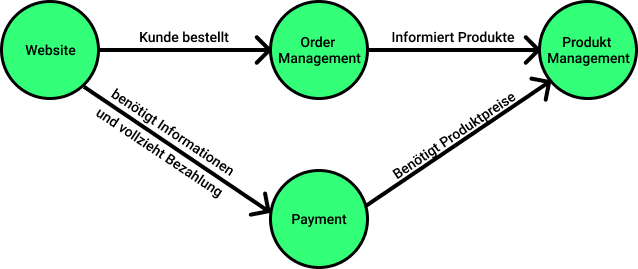
\includegraphics[width=1.0\linewidth]{img/prozess_eCommernce.png}
	\caption[Prozess Online-Shop]{Vereinfachter Prozess eines Online-Shops mit vier Komponenten\\ Quelle: Eigen}
	\label{fig:prozess_online_shop}
\end{figure}

In Abbildung \vref{fig:prozess_online_shop} ist der Prozess beschrieben. Es wird dabei nur ein einfacher Bestellprozess betrachtet. Ein Kunde bestellt auf einer Website bestimmte Produkte. Im Order-Management werden dann die Informationen zu entsprechenden Produkte, die zu dieser Bestellung gehören aus dem Produkt-Management angefordert. Mithilfe der Produktinformationen kann dann im Bezahlbereich ein Endpreis für den Nutzer kalkuliert werden. Die dort generierten Informationen können dann wieder der Website zur Verfügung gestellt werden, damit der Nutzer einen Bezahlvorgang einleiten kann.

\subsection{Monolithen}
Wird nun ein Entwicklerteam damit beauftragt ein System auf Basis dieses Prozesses zu implementieren so kann ein \textbf{monolithischer Ansatz} gewählt werden. Eine ebenfalls vereinfachte Architektur könnte für den oben beschreibenen Prozess folgendermaßen aussehen:

\begin{figure}[h]
	\centering
	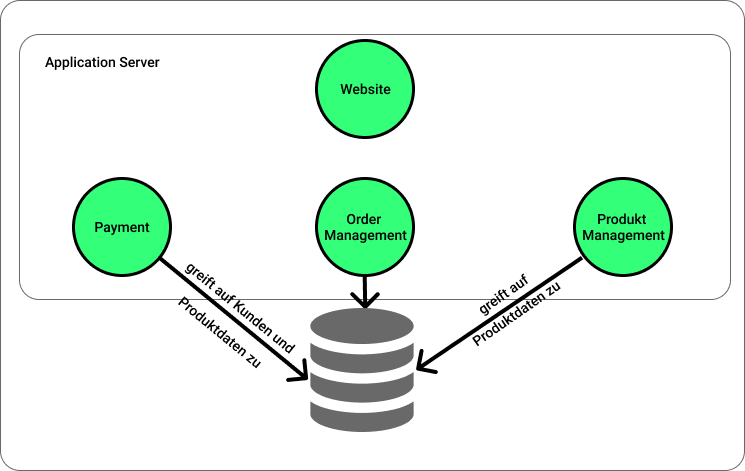
\includegraphics[width=1.0\linewidth]{img/monolitische_architektur.png}
	\caption[monolitische Architektur]{Abbildung des Prozesses mithilfe eines monolithischen Ansatzes\\Quelle: Eigen}
	\label{fig:monolithic_arch}
\end{figure}

Die in \vref{fig:monolithic_arch} beschriebene Architektur hat einige Eigenschaften, welche sie zu einer monolithischen Architektur werde lassen. Dazu gehört unter anderem die Tatsache, dass der Prozess in verscheidene Komponenten oder Module unterteilt wird, welche alle zusammen die Applikation bilden. Zusätzlich greifen alle Komponenten, da sie als eine Einheit deployt werden auf dieselbe Datenbank zu. Sowohl die Tatsache, dass es nicht in einzelne Services sonder Komponenten unterteilt wurde und das sich eine gemeinsame Datenbank geteilt wird stellen Merkmale dar, welche auf eine monolithische Architektur schließen lassen. Ein Vorteil dieses Ansatzes ist, dass die Kommunikation zwischen den verscheidenen Komponenten sehr einfach ist, da diese meistens auch logisch als \textit{ein Programm} ablaufen. So kann das Order-Management Daten anfordern indem es eine Methode im Produkt-Management aufruft. Ein \textbf{Nachteil} dieses Ansatzes besteht aber darin, dass eine sehr starke Kohäsion und Abhängigkeit von der spezifischen Implementierung einer Komponente besteht. So kann beispielsweise das Order-Management nur ausgestausch werden, wenn unter viel Aufwand auch alle anderen Komponenten in dem Monolithen angepasst werden. 

\begin{definition}[Monolith]
	Monolithen lassen sich anhand folgender Eigenschaften definieren: \autocite[S. 3]{microservice_enterprise}
	\begin{enumerate}
		\item Monolithen werden als einzelne Einheit entworfen, entickelt und deployt. Dies bringt mit sich, dass sie oftmals eine enorme Komplexität erreichen, welche nicht gut zu überblicken ist.
		\item Die einzelnen implementierten Businessfunktionen können nicht einzeln skaliert oder aktualisiert werden. Alle Komponenten sind also an zentrale Deployments des gesamten Monolithen gebunden, auch wenn nur eine Komponente aktualisiert werden muss.
		\item Die initiale Wahl einer Programmiersprache kann später nichtmehr oder nur sehr schwer wieder geändert werden, da jede einzelne Folgeentscheidung auch auf Basis dieser Wahl getroffen wurde.
		\item Bei Instabilität einer einzelnen Komponenten besteht Gefahr, dass die gesamte Applikation einen Fehler erleidet und nichtmehr funktionsfähig ist.
	\end{enumerate}
\end{definition}

\subsection{SOA und ESB}

Eine Lösung für die Nachteile, die ein Monolith mit sich bringt sollte mithilfe der \ac{SOA} erreicht werden. Die \ac{SOA} versucht die große, schwer skalierbare und stark zusammenhängende Einheit eines Monolithen aufzubrechen in kleine \enquote{self-contained} Services. Diese Services haben einen klar definierten Aufgabenbereich und besitzen ein wohldefiniertes Interface, welches \textbf{unabhängig} von der unterliegenden Implementierung ist. Dies löst bereits mehrere Probleme, welche in einem Monolithen vorhanden waren. So kann nun durch die lose Kopplung zwischen den Services (Komponenten in dem Monolithen) eine individuellere Skalierbarkeit erreicht werden. Jetzt stehen aber nicht mehr nur ein zentraler Endpunkt wie bei dem Monolithen zur Verfügung der von einem Client angesprochen werden kann. Es kommt auch die Frage auf, wie bestimmt werden kann, welcher Instanz eines Service angesprochen wird, wenn dieser in mehreren Replikaten vorliegt. Um unter anderem diese zwei wichtigen Punkte zu lösen wird die \ac{SOA} meistens nur in Verbindung mit einem \ac{ESB} verwendet.

Unter einem \ac{ESB} kann man sich vereinfacht eine Art intelligenten Load-Balancer vorstellen. Zu den klassischen Aufgaben eines \ac{ESB} gehören unter anderem die Weiterleitung der Anfragen eines Clients zu den richtigen Services. Der Grund warum es sich bei dem \ac{ESB} um einen Art intelligenten Load-Balancer handelt ist, weil er zusätzlich die Fähigkeit besitzt einzelne Services zu zusammengesetzten logischen Einheiten zu kombinieren. Wie diese Services kombiniert werden obliegt dabei dem Implementierenden, welcher es auf Basis des zu implementirenden Prozesses entscheiden kann. Zusätzlich können in einem \ac{ESB} noch Funktionen wie beispielsweise Authenthifizierung von Clients oder auch Monitoringfunktionen eingebaut werden.\\
Das oben eingeführte Beispiel könnte umgesetzt in einer \ac{SOA} folgendermaßen umgesetzt werden:
\begin{figure}[]
	\centering
	\caption{TODO: Hier kommt noch das Bild der SOA Arch hin}
\end{figure}

Diese nächste \enquote{Entwicklungsstufe} auf dem Weg zur Microservicearchitektur lässt sich also mithilfe folgender Eigenschaften definieren:

\begin{definition}[SOA und ESB]
	Im Rahmen der \ac{SOA} ist ein Service mit folgenden Eigenschaften definiert: \autocite[S. 4]{microservice_enterprise}
	\begin{enumerate}
		\item Ein Service ist eine eigenständige Implementierung einer wohldefinierten Businessfunktion, welcher über das Netzwerk erreichbar ist. Sie sind lose gekoppelt und verfügen über ein wohldefiniertes Interface über welches sie nach außen hin ansprechbar sind, somit sind sie implementierungsunabhängig. Services stellen die Grundbausteine innerhalb der \ac{SOA} dar.
		\item Zusammengesetzte Services können mithilfe auf Basis bestehender Services generiert werden und erben alle Eigenschaften, die ein Service auch hat.
		\item Services können dynamisch registriert werden. Es ist oftmals für den Client nicht von relevanz den genauen Ort eines Services zu kennen, da diese im Rahmen einer Service-Registry in Form von Metadaten vorliegen.
	\end{enumerate}
	Dem \ac{ESB} fällt dabei die Rollen eines intelligenten Mittelsmann (\enquote{smart Pipeline}) zu. Er besitzt die Möglichkeit Services zusammenzufassen und sich um die Sichtbarkeit, sowie die zusätzliche Bereitstellung von Funktionen zu kümmern. Er stellt einen zentrale Schnittstelle zwischen den einzelnen Services und der \enquote{Außenwelt} innerhalb der \ac{SOA} dar.
\end{definition}

\subsection{Der letzte Schritt - die Microservicearchitektur}

%%%%%%%%%%%%%%%%%%%%%%%
%	OBSERVABILITY	  %
%%%%%%%%%%%%%%%%%%%%%%%
\section{Observability}

Der Begriff und der Nutzen von Observability für Services lässt sich anhand der folgenden Zitate sehr gut nachvollziehen.

\begin{quote}
	\enquote{Collecting data is cheap, but not having it when you need it can be expensive.}\autocite[S. 373]{microservice_enterprise} - \textit{\citeauthor{microservice_enterprise}}

	\enquote{Observability is the measure of how well internal states [...] of a system can be inferred by knowledge of its external outputs [...].}\autocite[S. 35]{Yordanova2016} - \textit{\citeauthor{Yordanova2016}}
\end{quote}

Innerhalb einer jeden Technologie wird uns durch Standards \marginpar{CNCF} eröglicht wichtige Einsichten in Services zu erhalten. Wird jedoch darauf verzichtet Daten aus einem Service zu sammeln, so kann es im Fehlerfall die Konsquenz haben, dass Fehler erst garnicht entdeckt oder bemerkt, geschweige denn gelöst werden. Die Observability von Services, welche innerhalb einer Applikation genutzt werden ist also von essenzieller Bedeutung. Nun kommt die Frage auf, was genau ist Observability? Welche Aspekte meines Service muss ich überwachen, um zuversichtlich sien zu können, einen Fehlerfall schnell bemerken zu können und diesen dann durch die gesammelten Daten schnell analysieren zu können?\\
In \citetitle{Sridharan2018} wird beschrieben, wie sich Services in verteilten Systemen observieren lassen. Dazu nimmt der Autor eine Unterteilung in drei Säulen vor.

\begin{definition}[Die drei Säulen der Observability]\autocites[Chapter 4: Three Pillars of Observability]{Sridharan2018}[S. 373f]{microservice_enterprise}
	Um erfolgreich auf interne Zustände schließen zu können, müssen Daten existieren auf deren Basis Schlussfolgerungen gezogen werden können. Diese Daten werden aus drei verschiedenen Bereichen erhoben:

	\newcounter{pillarsCounter}

	\begin{enumerate}
		\item \textbf{Logging:}\\
		Das Zeil des Loggings besteht darin, Ereignisse zu dokumentieren. Es ist dabei nicht von Bedeutung, um welche Events es sich handelt. Zusätzlich zu den eigentlichen Daten des Ereigisses, welche unterschiedlichster Art sein können, ist es möglich Metadaten zu loggen, welche dem Ereigis zusätzlichen Kontext verleihen oder einen sonstigen Mehrwert bieten. Dazu gehören z.B. Information zum Zeitpunkt des Ereigisses (\textit{timestamp}), Ergebnis des Ereigisses (\textit{status}), usw. 
		
		Ein Vorteil des Loggings bestehen unter anderem darin, dass diese extrem einfach zu generieren sind. Ein Nachteil des Loggings besteht darin, das Logs an sich keine zusätzliche Aussagekraft haben, außer ihrem direkten Inhalt. Es ist schwer rein anhand von Logs ein komplexes Fehlerbild in einem verteilten System zu finden und korrekte Maßnahmen zur Behebung zu treffen.
		\item \textbf{Metriken:}\\
		Metriken stellen eine numerische representation von Daten dar, welche über bestimmte Zeitintervalle gemessen wurden. Metriken können also als Indikator verwendet werden, wie gut oder schlecht ein Services performt. Populäre Metriken wären z.B. die Anzahl der Anfragen, die ein Service in einer Minute verarbeitet, oder die durschnittliche Antwortzeit eines Service (seine Latenz). Das zweite Beispiel zeigt sogar ein Zusammenspiel zwischen zwei Säulen auf. Diese Metrik kann als abgeleitete Eigenschaft aus Daten des Loggings interpretiert werden, da die Latenz als Differenz zwischen dem Zeitpunkt der Anfrage und dem Zeitpunkt der Antwort ist.
		\setcounter{pillarsCounter}{\value{enumi}}
	\end{enumerate}

	\textbf{Logging} kann also als datenaggregierende Säule angesehen werden. \textbf{Metriken} hingegen nutzen (unter anderem) die aggregierten Daten, um neue wertvollere Informationen abzuleiten. Die Kombination zwischen diesen beiden Säulen bietet einem Aussenstehenden einen guten Einblick in den internen Zusatand \textit{eines} Services. Wie bereits bei der Defintion eines Microservices erwähnt ist es aber nicht unüblich hunderte kleine Services beobachten zu müssen. Es wäre allerdings sehr unpraktisch nur die einzelnen Services in Isolation zu betrachten, da es sich um stark vernetzte und voneinander abhängige Services handelt. Deshalb existieren noch eine dritte Säule, um auch serviceübergreifend Daten zu aggregieren und diese zu verwertbaren Informationen umzuwandeln.

	\begin{enumerate}
		\setcounter{enumi}{\value{pillarsCounter}}
		\item \textbf{Tracing:}\\
		Betrachtet man die bisherigen Säulen, so lässt sich ein Trend auf der Betrachtungsebene feststellen. Das Logging fokussiert sich auf die Sammlung der Daten einzelner Ereignisse, der kleinsten Einheit. Die Metriken arbeiten nun ereignisübergreifend und wandeln die Daten zu nutzbaren Informationen um, damit Einsichten in das Verhalten eines Services vorhanden ist - die mittlere Einheit. Der nächste logische Schritt wäre nun, da Services in einem verteilten System miteinander vernetzt sind, eine Anfrage von Beginn bis zur endgültigen Antwort serviceübergreifend zu observieren, quasi eine End-to-End Betrachung. Genau diese Betrachtung wird mithilfe von Tracing ermöglicht. Eine \textit{Trace} (\enquote{Spur}) ist eine Liste zusammenhängender, verteilter Eregnisse, welche als Repräsentant einer End-to-End Anfrage angesehen werden können.
	\end{enumerate}

\end{definition}
Mithilfe dieser drei Säulen ist es nun einem Aussenstehenden möglich auf \enquote{die inneren Zustände eines Systems auf Basis seiner Ausgaben} zu schließen. Dazu ein kurzes Beispiel:\\
Es wird ein Fehler bei einer Anfrage regisitriert. Der dafür zuständige Mitarbeiter kann nun mithilfe des \textbf{Tracings} feststellen um welches Request es sich handelt. Dabei erkennt er, welche Services als Ursache für den Fehler infragekommen. Im nächsten Schritt kann er sich einzelne \textbf{Metriken} der Services ansehen, um eventuell eine Anomalie festzustellen. Im letzten Schritt kann er durch ansehen der \textbf{Logs} eine genaue Fehlerursache feststellen.


\section{Governance}

Eine Einführung von Microservices in ein Unternehmen kann sehr viele Vorteile besitzen. Sollte sich ein Unternehmen dazu entschließen, von der bisherigen Architektur auf eine Microservicearchitektur umzustellen, bringt dies auch einige Herausforderungen mit sich. Sind in einem Unternehmen bisher nur Monolithen bekannt, so kann die durch Microservices hinzukommende Komplexität schnell zu einem Problem werden. Zumal es sich hierbei um eine immense Anzahl neuer Services, am Beispiel von Netflix sogar mehr als 700 handeln kann. Es stellt sich nun also auch aus der Sicht eines Unternehmens die Frage, wer ist zuständig für einen bestimmten Service? Wie hängen die Services zusammen? Welche Services sind überhaupt vorhanden? Wie können Fehler in einzelnen Services erkannt werden und deren Auswirkungen bestimmt werden?

All diese Frage gehören zu dem Bereich der Microservice-Governance und sollten sich im Vorfeld eines Umstiegs auf eine Microservicearchitektur klären lassen. In \citetitle{microservice_enterprise} wird unter der Governance folgendes verstanden:

\begin{definition}[Dezentralisierte Governance]
	Die dezentralisierte Governance setzt sich unter anderem aus vier Kernmodulen \autocite[S. 154]{microservice_enterprise} zusammen. Dabei handelt es sich um:
	\begin{enumerate}
		\item die Observability
		\item eine Service-Registry und Service-Discovery
		\item das API-Management und
		\item die Entwicklungszyklen
	\end{enumerate}
	Diese vier Kernmodule sind innerhalb eines Microservice Ansatzes nicht dezentral verwaltbar. Weitere Bestandteile eines Microservice, welche im Bereich der Governance liegen sind design, development und deployment eines Services. Hierfür sollt es keine zentrale Verwaltung geben,\autocites[S. 154]{microservice_enterprise} [Decentralized Governance]{FowlerMicrservices}sonder die Veranwtortlichkeit sollte im entwickelnden Team liegen.
\end{definition}

Eine dezentralisierte Governance wie sie bei Microservices genutzt wird hat einie Vorteile gegenüber dem früheren komplett zentrierten Governance-Ansatz. So kann zum Beispiel für jeden Anwendungsfall die Tools von dem zuständig Team selbst gewähl werde und es wird nicht von einer unternehmensweiten Grundsatzentscheidung bestimmt, dass nur ein bestimmer Technologieverbund genutzt werden kann. Trotz dieser Freiheit bleiben wichtige Elemente wie die Observability eines Services in einem zentralisierten skalibaren Service verfügbar, sodass wichtige Daten immer von allen Services zur Verfügung stehen. Hier ist eine zentrale Vorschrift sogar förderlich, da so sichergestellt wird, dass keine \enquote{Insights} verloren gehen, da ein Subset der im Unternehmen vorhanden Service andere Tools für das Monitoring benutzen als der Rest.

Im Rahmen dieser Arbeit wird in Kaptiel \vref{chap:KonzepTool} ein Tool vorgestellt, welches ein Problem im Bereich der Governance in Verbindung mit Elementen aus der Observability lösen soll. Dabei ist eine weitere zentralisiert verwaltete Komponente der Governance relevant. Dabei handlet es sich eine Art Service-Registry mit erweiterter Observability Funktionalität.

\section{Betrachtung bestimmter Gesichtspunkte im Rahmen der Governance und Observability}

Viele Konzepte, welche für Microservices essenziell sind stellen mit einem strengen Blick auf die Governance und die Observability eine Herausforderung dar. So werden im folgenden Teil einige dieser Konzepte vorgestellt und die damit verbundenen Probleme erläutert. Diese Probleme müssen mithilfe von Tooling oder eventuell sogar Designentscheidungen während der Softwareentwicklung verhindert werden.

\subsection{Design for Failure}
Bei Design for Failure \autocite{FowlerMicrservices} handelt es sich um ein Kernprinzip, welches bereits von \citeauthor{FowlerMicrservices} in seiner Zusammenstellung zu dem Architekturprinzip Microservice in \enquote{\citetitle{FowlerMicrservices}} vorgestellt wurde. Die Idee hinter diesem Prinzip ist, dass Fehler immer, erst Recht im Softwareumfeld unvermeidbar sind. Deshalb müssen 


Design for Failure, aber wie bekomme ich es mit? Wie reagiere ich im Fehlerfall? Was muss getan werden, und wie groß sind die Auswirkungen wenn einer meiner tausend Microservices ausfällt? Diese und viele weitere Fragen müssen sich DevOps und Software-Engerneering Teams oftmals stellen, wenn sie sich in einer dezentralisierten Microservicearchitektur befinden. Es ist oftmals ein tiefes Verständnis des Zusammenspiels der einzelnen Services nötig um heruaszufinden, ob ein Fehler von eigenen Service kommt, oder ob es aufgrund eines Fehlers in einem anderen Service kommt. Das ultimative Ziel ist es dabei herauszufinden was das Problem ist und dieses auch schnellstmöglich zu beheben, sodass für den Endnutzer keine Merkbaren folgen auftreten. Microservices folgen dem Prinzip \enquote{Design for Failure}, sodass eine Recovery möglich ist und ein operatives Business aufrecht erhalten werden kann. Trotz dieser hervorragenden Prämisse reicht ein \enquote{Design for Failure} alleine nicht aus. \enquote{Ein System ist nur so schlau wie das schwächste seiner Bestandteile}. Microservices mit dem Ziel kleiner dezentralisierter Services, welche einen spezialisiert sind auf eine bestimmte aufgabe innerhalb eines BusinessProzesses haben ironischerweise eine ihrer größten Schwäche in der Kommunikation miteinander. Es müssen Standards etabliert werden, sodass ServiceOwner einen wartbaren und funktionsfähigen Service entwickeln können. Es muss einen Software-Engeneer an einer Stelle ein Fehler unterlaufen und aufgrund der starken Kohäsion und Abhängigkeit der einzelnen Services unterneinander kann eine Reihe wichtiger Businessfunktionen davon betroffen sein.

Kein Problem - \enquote{Design for Failure}. Ein Service fällt aus und ist darauf ausgelegt sich selbst wieder zu reaktivieren. Alle anderen Services können einen ausfall händeln. Soweit die Theorie. In der Praxis ist das leider nur allzuoft nicht der Fall. Innerhalb der Microservice-Governance steht der Aspekt der dezentralisierten Entscheidungsfindung im Vordergrund. Das bedeutet, dass jedes Team das fachliche und unternehmerische Know-How zugesprochen wird das beste Tool und die beste Technologie für die von ihnen zu lösende Aufgabe zu wählen. Fängt ein Team nun an diese Aufgabe zu lösen, so benötigt er oftmals Informationen aus anderen Microservices, um seine Aufgabe zu erfüllen. 


\begin{center}
	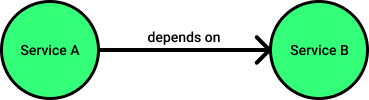
\includegraphics[width=0.55\linewidth]{img/service_dependency.png}
\end{center}

Es entsteht also eine Abhängigkeit zwischen zwei Microservices. Ebendieser angefragte Microservice benötigt aber wiederum einen anderen Service, um die angeforderte Information generieren zu können. Es entsteht also schon eine Kette von Abhängigkeiten. Was passiert, wenn ein Glied dieser Kette einen Fehler wirft? 

\Large Hier kommt ein Bild von einem Fehler in einer Microsericekette

\normalsize

Kein Problem - \enquote{Design for Failure}. Ein Architekt muss in der Planung seines Services die Möglichkeit haben, das Risiko und die Auswirkungen einen Ausfalls sowohl seines eigenen Services, als auch seiner Abhängigkeiten einschätzen zu können. Diese Einschätzung sollte auf Daten basieren, welche sowohl Information bisheriger Ausfälle und deren Ursachen enthalten als auch Ausblicke geben können auf den aktuellen Stand und eventuelle zukünftige Ausfälle.

Wie bereits Eingangs erwähnt ist bei der Betrachtung dieses Prinzips die Brille der Governance und Observability aufgesetzt. Es ist ein wichtiger Bestandteil die Services innerhalb einer Unternehmensarchitektur so aufzubauen, dass diese trotz eins Fehlers ordnungsgemäß weiterlaufen und die Fähigkeit zur Recovery besitzen. Dieses Prinzip ist sogar dafür Veranwtortlich, dass Microservicepioniere wie Netflix innerhalb der Observability eine eigene, vierte Säule zu etablieren. Dabei handelt es sich um das sogenannte Chaos-Testing. Um dies kurz zu erläutern: Dabei handelt es sich um einen eigenen \enquote{Service}, welcher auf Basis von Chaos-Experimenten produktive Services ausschaltet und so die Recovery ebendieses Services und auch der davon abhängigen Services überprüfen kann. Dies bringt viele Vorteile mit sich und sorgt auch dafür, dass Services gut entwickelt sind. Diese Idee, wie das bewusste Einführen von Fehlern die generelle Qualität von Services verbessern kann, wird näher in \citetitle{AntifragileOrganization}\autocite{AntifragileOrganization} beschrieben.
